% Kinematic fitting at ANKE
Разработанное расширение было использовано авторами для кинематического фита в реакции $pp \to pp$ на данных, полученных на спектрометре ANKE (Jülich, Germany)\cite{anke}.

% На рисунке \eqref{anke_scheme} можно видеть, что в процессе прохождения протонного пучка через установку часть протонов может отклоняться от направления основного пучка и не фиксироваться установкой, таким образом при анализе данных эксперимента мы можем столкнуться с разницей зафиксированных энергий и количества вещества, вступившего в реакцию с данными, полученными на выходе. Восстановить долю таких ``потерянных'' протонов мы можем, используя инвариант Лоренца $\left|\boldsymbol{P}^{(4)}_\mathrm{beam}+\boldsymbol{P}^{(4)}_\mathrm{targ}-\boldsymbol{P}^{(4)}_p\right|^2 = m_p^2$.

Рассмотрим область мишени, изображённую на рис.~\eqref{anke_scheme}, где происходит упругое $pp$ взаимодействие и один из протонов регистрируется в координатных камерах Fd.
Результатом является набор измеренных значений координат кластеров ${C_i:m }$ c ошибками ${\delta C_i}$.

\begin{figure}[h]
\centering
\centering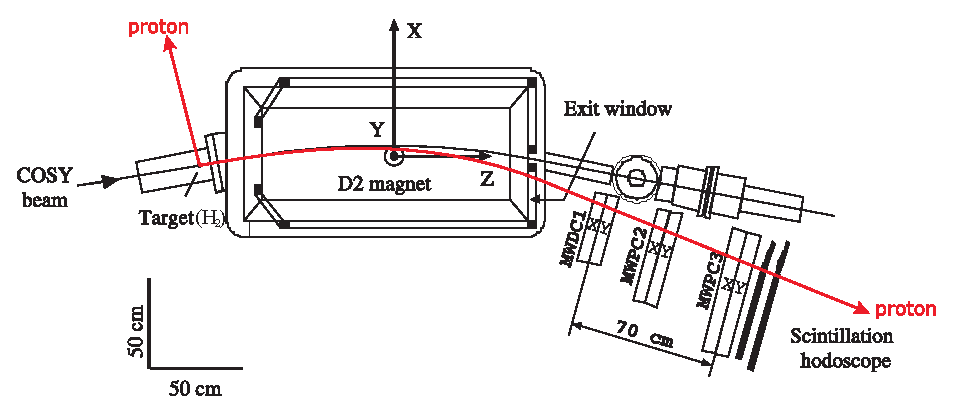
\includegraphics[width=0.8\textwidth]{pics/setup_.eps}
\caption{
Схема прохождения протонного пучка через установку ANKE.
}
\label{anke_scheme}
\end{figure}

Истинная координата трека $C_i$ есть функция $C_i = C_i (V, P)$, где вектора $V, P$ содержат координаты вершины и компоненты импульса. Далее делается разумное предположение, что разность $C_i - C_i^m$
распределена по Гауссу с ошибкой ${\delta C_i}$. Функция правдоподобия совокупности измеренных координат
\begin{equation}
\label{FPC}
L_c \approx \prod_i \exp \left(\frac{−1}{2} \left(\frac{C_i - C_i^m}{\delta_{C_i}} \right)^2 \right) \ldotp \Delta C_i
\end{equation}

Функция правдоподобия для координат вершины (в предположении, что по каждой координате распределение Гауссово и они независимы; на самом деле функция плотности
вероятности распределения по координатам вершины может иметь более сложный вид):
\begin{equation}
\label{FPV}
L_c \approx \prod_i \exp \left(\frac{−1}{2} \left(\frac{V_i - V_i^m}{\delta_{V_i}} \right)^2 \right) \ldotp \Delta V_i
\end{equation}

Тогда совместная функция правдоподобия $L_G$ будет иметь вид:
\begin{equation}
 \label{FPG}
 L_G = L_V \ldotp L_C
\end{equation}
Наиболее точная оценка параметров будет получена путём минимизации общей функции правдоподобия $L_G$, однако, если нет информации об $L_V$, оценка параметров производится
% только по $L_C$.

TODO: Добавить, причем тут Polar CMS coordinates.


% \centering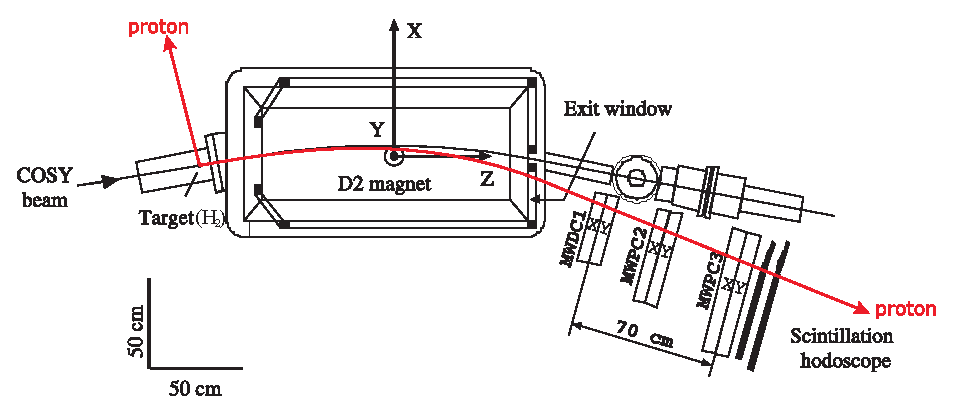
\includegraphics[width=0.8\textwidth]{pics/setup_.eps}

% \large
% \phantom{0}
% 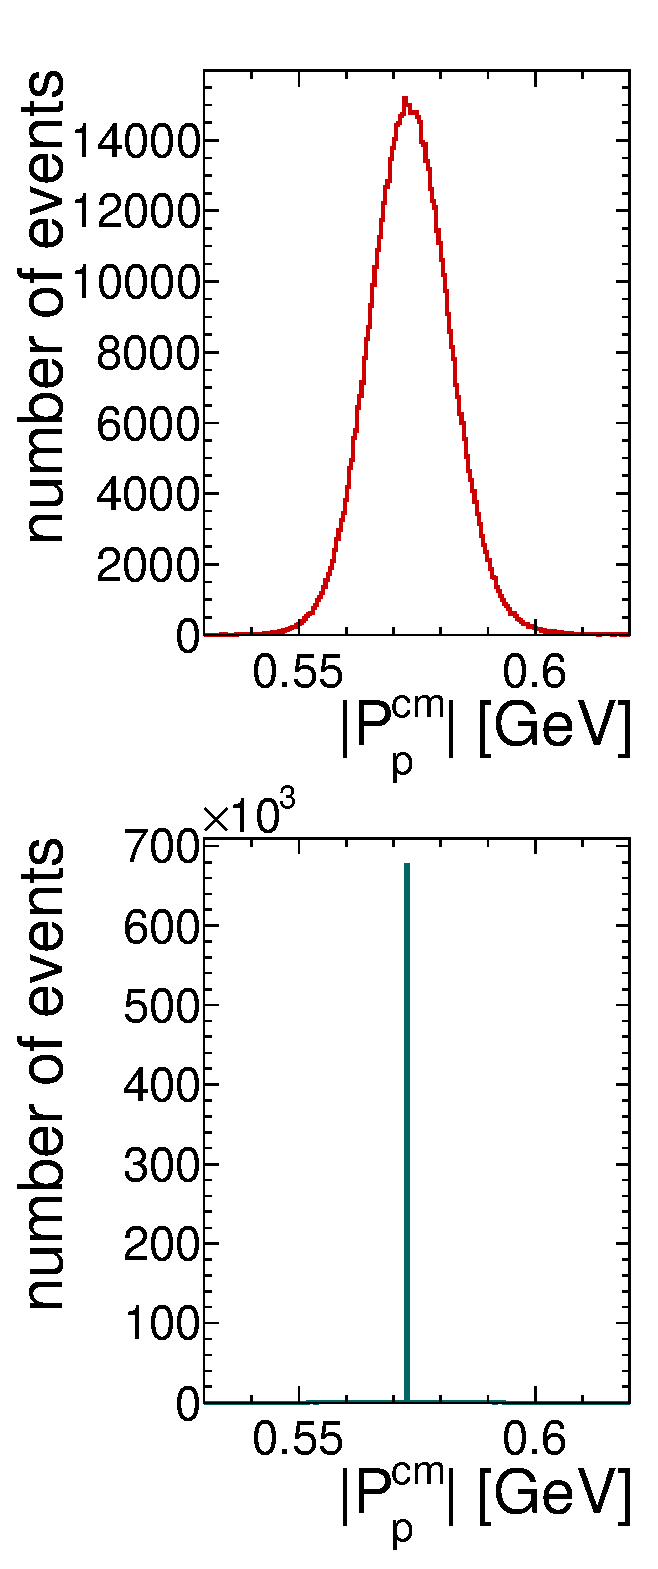
\includegraphics[height=0.7\textheight]{pics/drawMom.eps}
% \hfill
% 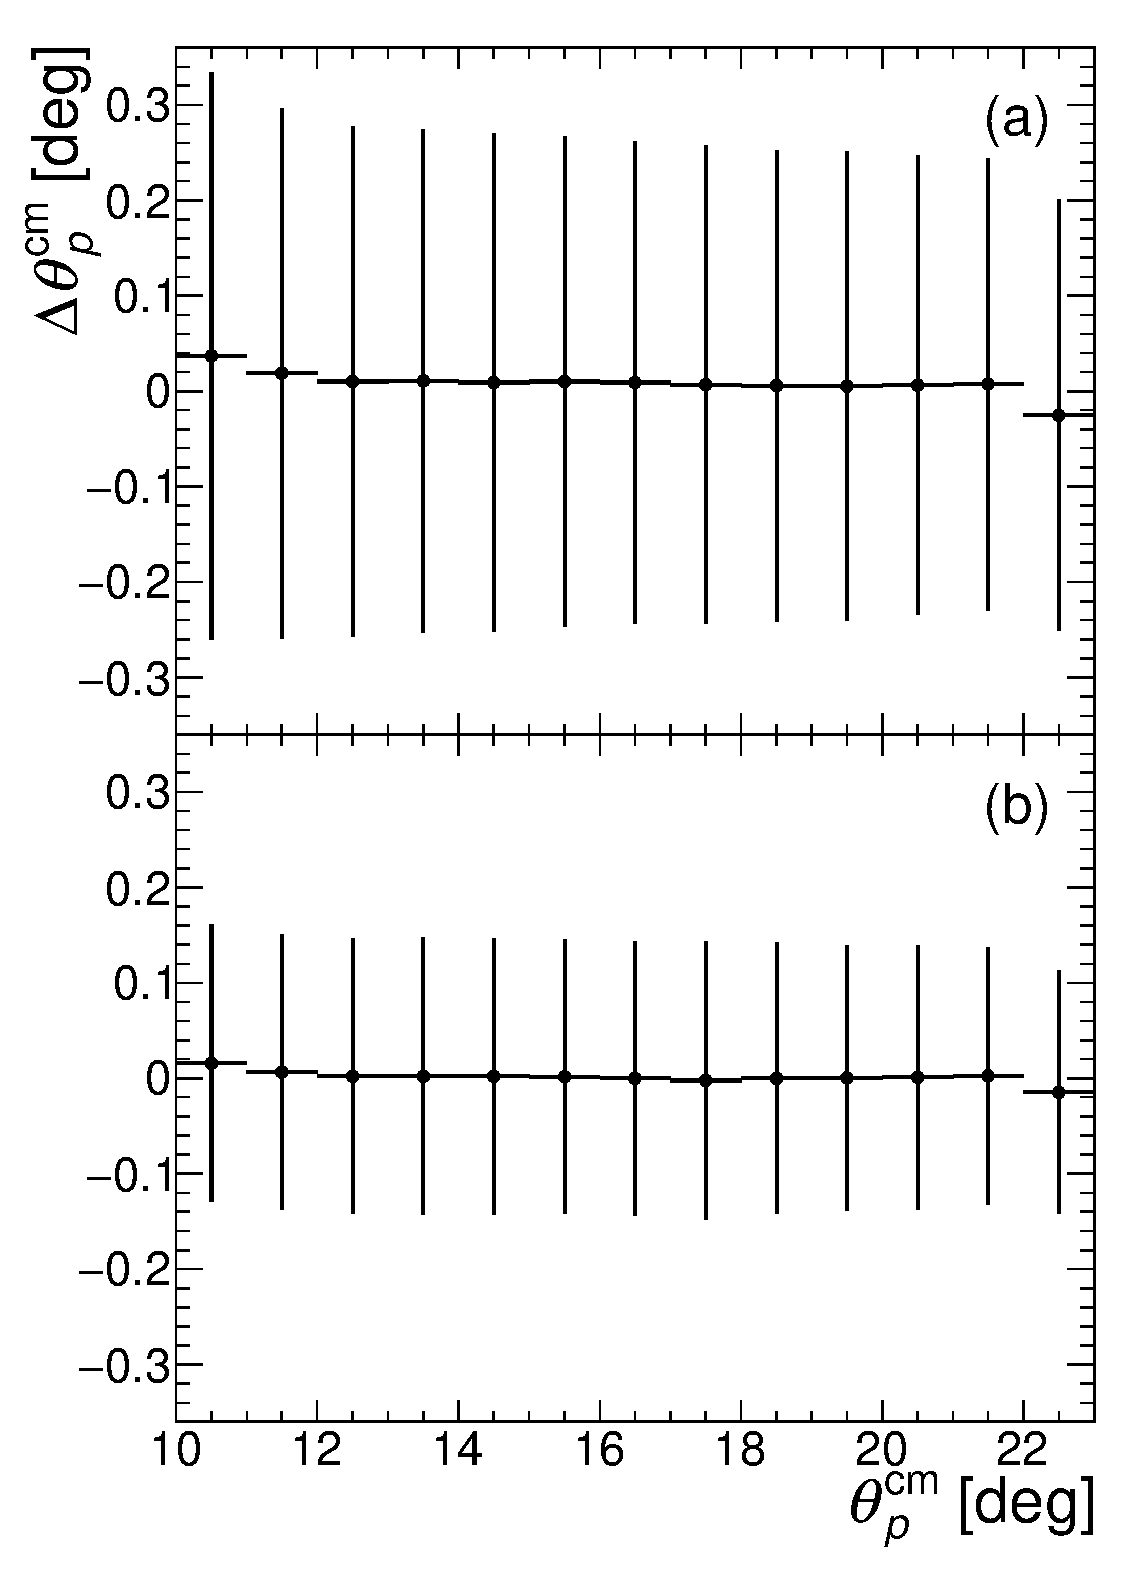
\includegraphics[height=0.7\textheight]{pics/drawTh.eps}
% \hfill
% % \hspace{1em}
% 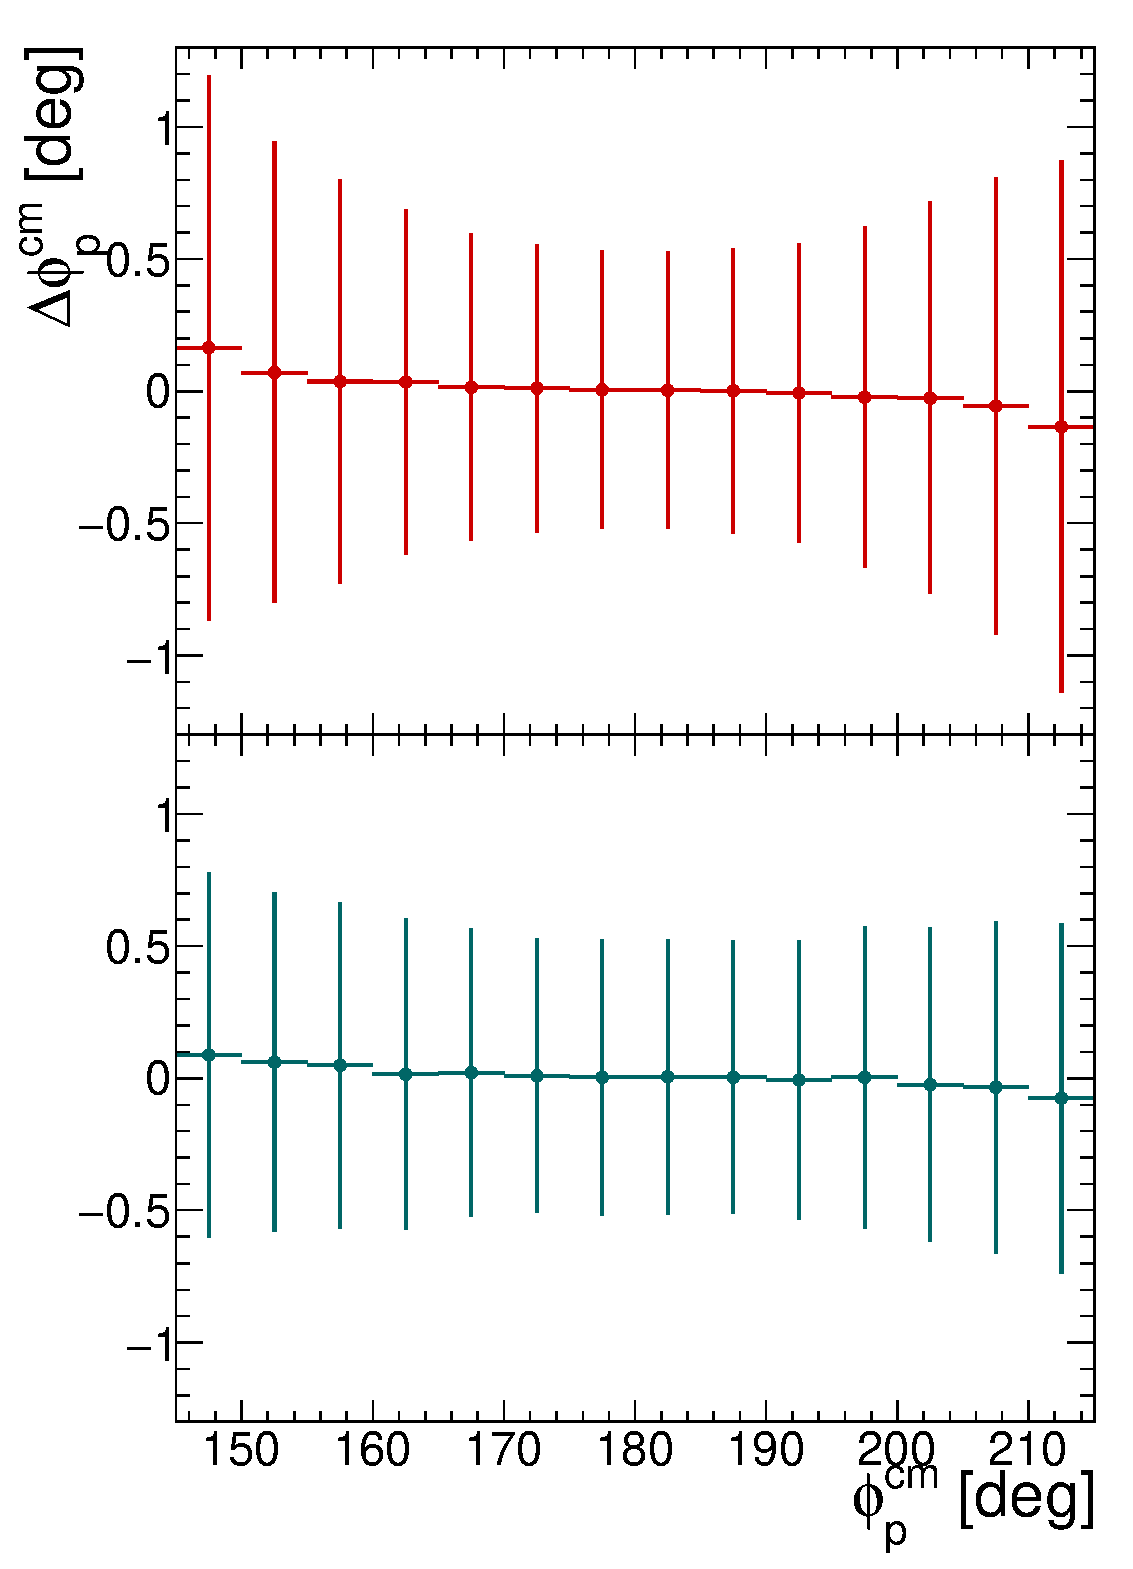
\includegraphics[height=0.7\textheight]{pics/drawPhi.eps}
% \hfill
% \phantom{0}

\begin{figure}[h]
\centering
\centering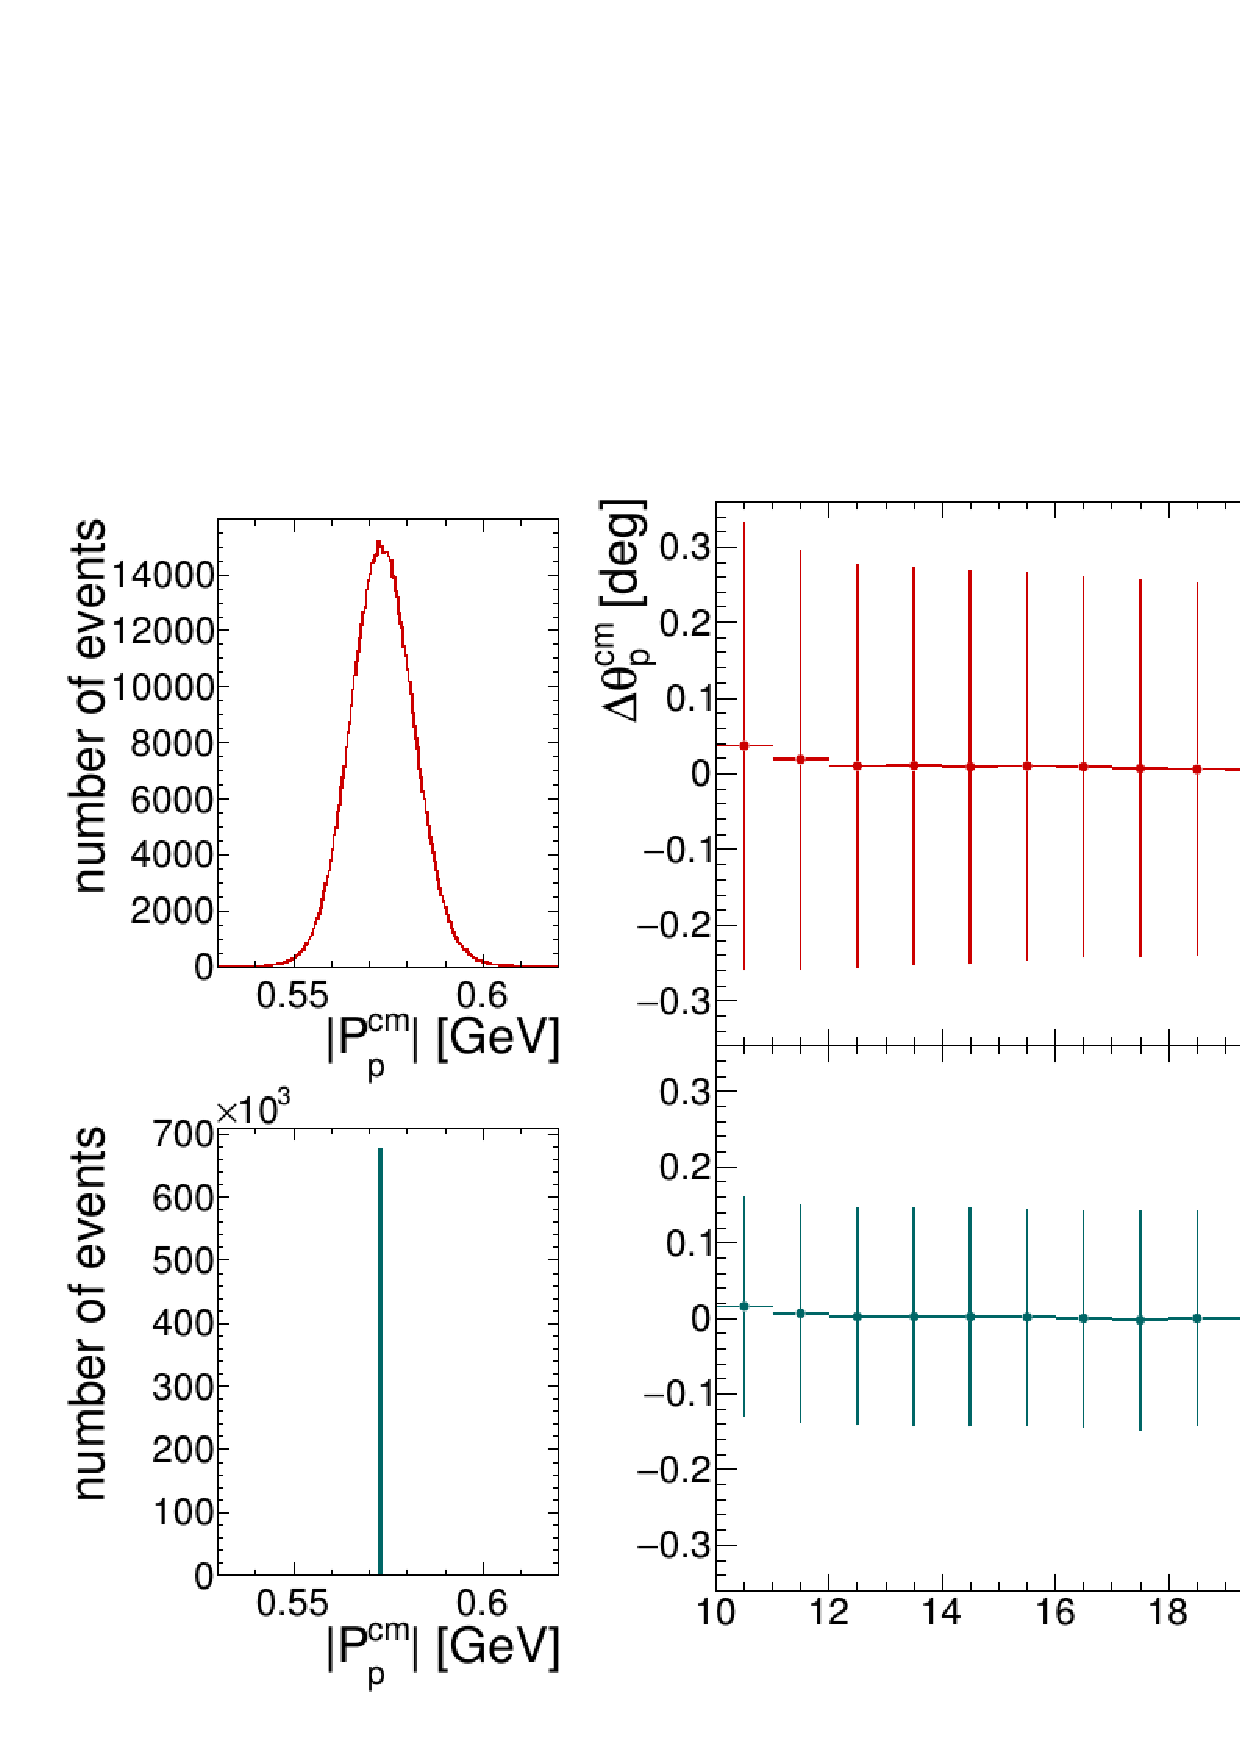
\includegraphics[width=0.9\textwidth]{pics/anke_errs.pdf}
\caption{
Errors of reconstructed proton momentum in polar coordinates $(|P_p^\mathrm{cm}|, \theta_p^\mathrm{cm}, \phi_p^\mathrm{cm})$ for the $pp \to pp$ reaction at ANKE, simulated for $T_\mathrm{beam} = 700$~MeV with and without kinematic fitting.
}
\label{anke_scheme}
\end{figure}
